\documentclass[11pt]{article}

% Font & ngôn ngữ tiếng Việt (pdfLaTeX)
\usepackage[utf8]{inputenc}
\usepackage[T5]{fontenc}


% Biblatex + biber
\usepackage[backend=biber, style=numeric-comp, autolang=other]{biblatex}

% Toán học & font Times
\usepackage{amsmath, amssymb, amsfonts, bm}

% Bảng biểu & căn lề
\usepackage{longtable}
\usepackage{array}
\usepackage{booktabs}

% Đồ họa & màu sắc
\usepackage{graphicx}
\usepackage{xcolor}
\usepackage{float}
\usepackage{subcaption}

% Liên kết & tham chiếu
\usepackage{hyperref}
\hypersetup{
    colorlinks=true,
    linkcolor=blue,
    urlcolor=red,
    pdftitle={Overleaf Example},
    pdfpagemode=FullScreen,
}

% Dấu tick và x
\usepackage{pifont}
\newcommand{\xmark}{\ding{55}}
\newcommand{\cmark}{\ding{51}}

% Tiêu đề tùy chỉnh
\usepackage{titling}
\setlength{\droptitle}{-10em}
\renewcommand{\maketitle}{%
    \begin{center}
        \fontsize{18}{20}\selectfont\textbf{Module 4 Tuần 3 \\[0.2em] LightXGBoost: A Practical Approach}\\[1em]
        \fontsize{14}{16}\selectfont Time-Series Team\\[0.5em]
        \fontsize{14}{16}\selectfont Ngày 19 tháng 9 năm 2025
    \end{center}
    \vspace{1.5em}
}

% Format section (không đánh số)
\usepackage{titlesec}
\titleformat{\section}{\normalfont\Large\bfseries}{}{0em}{}

% Code block
\usepackage{listings}
\definecolor{backcolour}{rgb}{0.95,0.95,0.92}
\lstset{
    backgroundcolor=\color{backcolour},
    basicstyle=\ttfamily\footnotesize,
    breaklines=true,
    numbers=left,
    numberstyle=\tiny\color{gray},
    captionpos=b
}

% Hộp màu
\usepackage[many]{tcolorbox}
\definecolor{lightgreenbox}{rgb}{0.85,0.95,0.85}
\newtcolorbox{summarybox}{
    colback=lightgreenbox,
    colframe=green!50!black,
    boxsep=5pt, arc=4pt,
    boxrule=0.5pt,
    left=10pt, right=10pt,
    top=10pt, bottom=10pt,
}


% Layout trang
\setlength{\topmargin}{-0.7in}
\setlength{\textheight}{9.25in}
\setlength{\oddsidemargin}{0in}
\setlength{\textwidth}{6.8in}

%%%%%%%%%%%%%%%%%%%%%%%%%%%%%%%%%%%%%%%%%%%%%%%%%%%%%%%%%%%%%%%%%%%%%%%%%%%%%
\begin{document}

\maketitle

\begin{summarybox}
Buổi học thứ 6 (ngày 19/9/2025) được chia thành 6 phần chính đi từ tổng quát đến chi tiết và công thức phía sau thuật toán này
    \begin{itemize}
        \item \textbf{Phần 1: Kĩ thuật Boosting}
        \item \textbf{Phần 2: Trực giác đằng sau AdaBoost }
        \item \textbf{Phần 3: Công thức toán đằng sau AdaBoost}
    \end{itemize}
\end{summarybox}

\section{Phần 1: Kĩ thuật Boosting}
Một cây quyết định (gọi tắt là DS) đơn lẻ thường không đủ mạnh để xử lý dữ liệu thực tế: nếu quá nông (1 node) thì chỉ dựa trên 1 đặc trưng duy nhất dẫn đến bỏ sót thông tin quan trọng hoặc nếu quá sâu (full decision tree) thì cây dễ ghi nhớ dữ liệu huấn luyện và mất khả năng khái quát. Chính vì hạn chế này mà các phương pháp \textbf{Essemble Learning} ra đời, nhằm kết hợp nhiều mô hình con để tận dụng ưu điểm và hạn chế nhược điểm của từng mô hình đơn, chi tiết thế nào mình cùng đi tiếp nhé.

 \subsection{Điểm yếu của Decision Tree}
Một cây quyết định quá nông gồm 1 node được gọi là \textbf{Stump} (dịch ra là 1 đoạn của cây) là chỉ chia dữ liệu dựa trên 1 đặc trưng duy nhất, ví dụ "nếu cân nặg $\geq 70$kg thì dự đoán bệnh tim = "có" cho thấy rõ ràng các yếu tố như tuổi, huyết áp và động mạch bị tắc, etc.. không được cân nhắc do thiếu nhánh để quyết định. Do đó, cây nông bị underfitting. \\

Ngược lại, 1 DS quá sâu có thể tạo ra hàng chục hoặc hàng trăm nhánh, quá phù hợp với dữ liệu huấn luyện nhưng lại thất bại khi dự đoán dữ liệu mới dẫn đến overfitting. 

\begin{figure}[H]
    \centering
    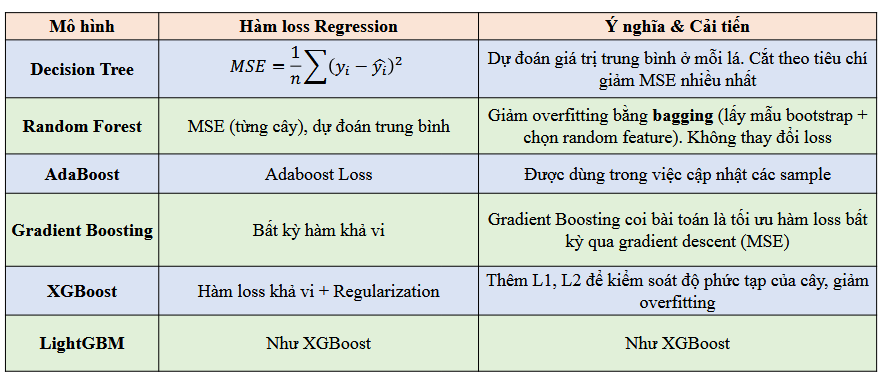
\includegraphics[width=0.7\linewidth]{images/loss_regr.png}
    \caption{Random Forest (nhiều Decision Tree vừa và sâu) vs Ada Boost (nhiều cây nông / Stump)}
\end{figure}
 

\end{document}
